% CHAPTER 2
\chapter{BACKGROUND AND LITERATURE REVIEW}
\label{chp:chapter2}

In this chapter, we cover the necessary background that is required to understand the overall study. Besides, we aim to review the relevant literature about post-transcriptional regulation. First, we discuss RBPs and their roles as regulators of post-transcriptional gene expression. We introduce the experimental and computational methods to detect their binding sites genome-wide. Then, we cover miRNAs which are also key regulators of post-transcriptional gene expression. We continue by introducing various methods for identifying miRNA sites. Next, we discuss RNA secondary structure which plays a crucial role in RBP-target and miRNA-target interactions. Finally, we review relevant studies that consider the effect of both RBPs and miRNAs in modeling post-transcriptional gene regulation.


\section{RNA-binding proteins}

RBPs are key factors in the regulation of gene expression at the mRNA level. RBPs bind to their target mRNAs and control several steps of RNA processing including splicing, stability, localization, and degradation \cite{dreyfuss_2002}. RBP-mRNA interactions form a multi-dimensional network. An mRNA can be bound by several RBPs. On the other hand, RBPs have hundreds of targets. More than 800 RBPs have been found in the human genome. Alternation in the activity of RBPs leads to dysregulations in PTR. These are associated with many diseases such as neurodegenerative disorders and cancer.

RBPs bind to their targets through one or more RNA-binding domains (RBDs). Some RBPs bind single-stranded RNA by direct readout of the primary sequence, whereas others recognize primarily the structure of the RNA \cite{drapper_99, zhu_2009}. There are also some RBPs which recognize their targets by both the sequence and the secondary structure \cite {johnson_2006}.

In recent years, several experimental methods have been developed to identify binding specificities of RBPs. These methods can be classified as \textit{in vitro} and \textit{in vivo} methods. \textit{In vivo} experiments are carried out within the cell. On the contrary, \textit{in vitro} studies are conducted in some controlled environment. The advantage of \textit{in vivo} methods are to model RBP-RNA interactions in their natural environment. However, this requires additional knowledge about the experimental condition in which the RBP is active. On the contrary, \textit{in vitro} methods identify RBP binding sites in non-biological conditions. However, this also enables querying non-genomic sequences such as variants of the wild-type binding sites and testing a wide range of interesting conditions (e.g. salts, pH). Below, we will discuss the widely-used \textit{in vitro} and \textit{in vivo} methods.

\subsection{In vitro methods}

Selection of ligands by exponential enrichment (SELEX) is a low-throughput method for \textit{in vitro} detection of RBP targets \cite{ellington_90}. This method selects high-affinity binding sequences from a randomized pool through multiple rounds of selection, purification, and amplification. This produces a set of high-affinity targets. One disadvantage of SELEX assay is that it reveals only the highest affinity RNA targets, which do not necessarily reflect the physiological targets.

RNAcompete is a method for rapid characterization of binding specificities of RBPs \textit{in vitro} \cite{ray_2009}. This method consists of three main steps: (i) generation of a custom-designed RNA pool containing short sequences; (ii) a single binding reaction to identify the RNAs bound by the tagged RBP of interest; and (iii) analysis of the microarray data to determine binding preferences of the RBP. This method is recently used to characterize the binding specificities of more than 200 RBPs from 24 diverse eukaryotes. Figure \ref{RNAcompete} shows the steps in RNAcompete method.

%\shorthandoff{=}
\begin{figure}[H]
   \centering
   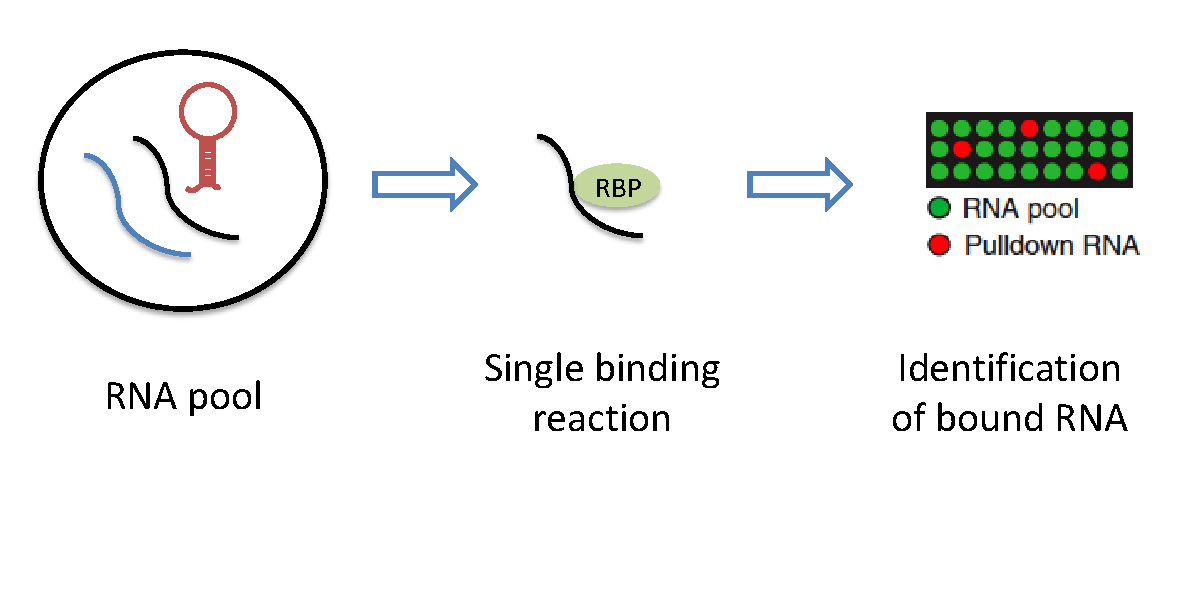
\includegraphics[width=0.6\textwidth,clip]{ch2_background/figures/RNAcompete.pdf}
\caption[Steps in RNAcompete method]{Steps of RNAcompete methods are simplified in this figure (Adopted from RNAcompete \cite{rnacompete_09})}
\label{RNAcompete}
\end{figure}
%\shorthandon{=}


\subsection{In vivo methods}

RNA immunoprecipitation (RIP) is a powerful high-throughput method which detects the association of an individual RBP with specific RNA. This method purifies RBP-mRNA complexes from cellular extracts and identifies protein-bound mRNAs using either a microarray (RIP-chip) or high-throughput sequencing (RIP-seq) \cite{keene_06, zhao_10}. The absence of cross-linking step in this method may lead to dissociation of RBPs from their targets \cite{mili_2004}.

Cross-linking and immunoprecipitation (CLIP or HITS-CLIP) method aims to eliminate the dissociation of RBPs mentioned in the previous method. Figure \ref{PARCLIP_HITSCLIP} shows the steps in PARCLIP and HITS-CLIP methods. This approach utilizes an ultraviolet light (UV) cross-linking step before immunoprecipitation. This enables a more stringent washing procedure to reduce contaminants and eliminate interactions that occur after cell lysis \cite{ule_05}. PARCLIP is a modified version of CLIP technique which uses photoactivatable ribonucleoside-enhanced cross-linking and immunoprecipitation. In this method, cross-linked sites are enriched with a thymidine to cytidine transition \cite{hafner_10}. This method identifies RBP binding sites by scoring T to C transitions in sequenced cDNA. T-C mutations are useful in identification of binding sites in high resolution. CLIP experiments identify the binding sites of a single RBP at a time while a recently proposed method called gPARCLIP (global PARCLIP) identifies the binding sites of all the RBPs that exist in the cell \cite{baltz_12}. However, this method is unable to detect and identify the particular RBPs that bind to a site.

%\shorthandoff{=}
\begin{figure}[H]
   \centering
   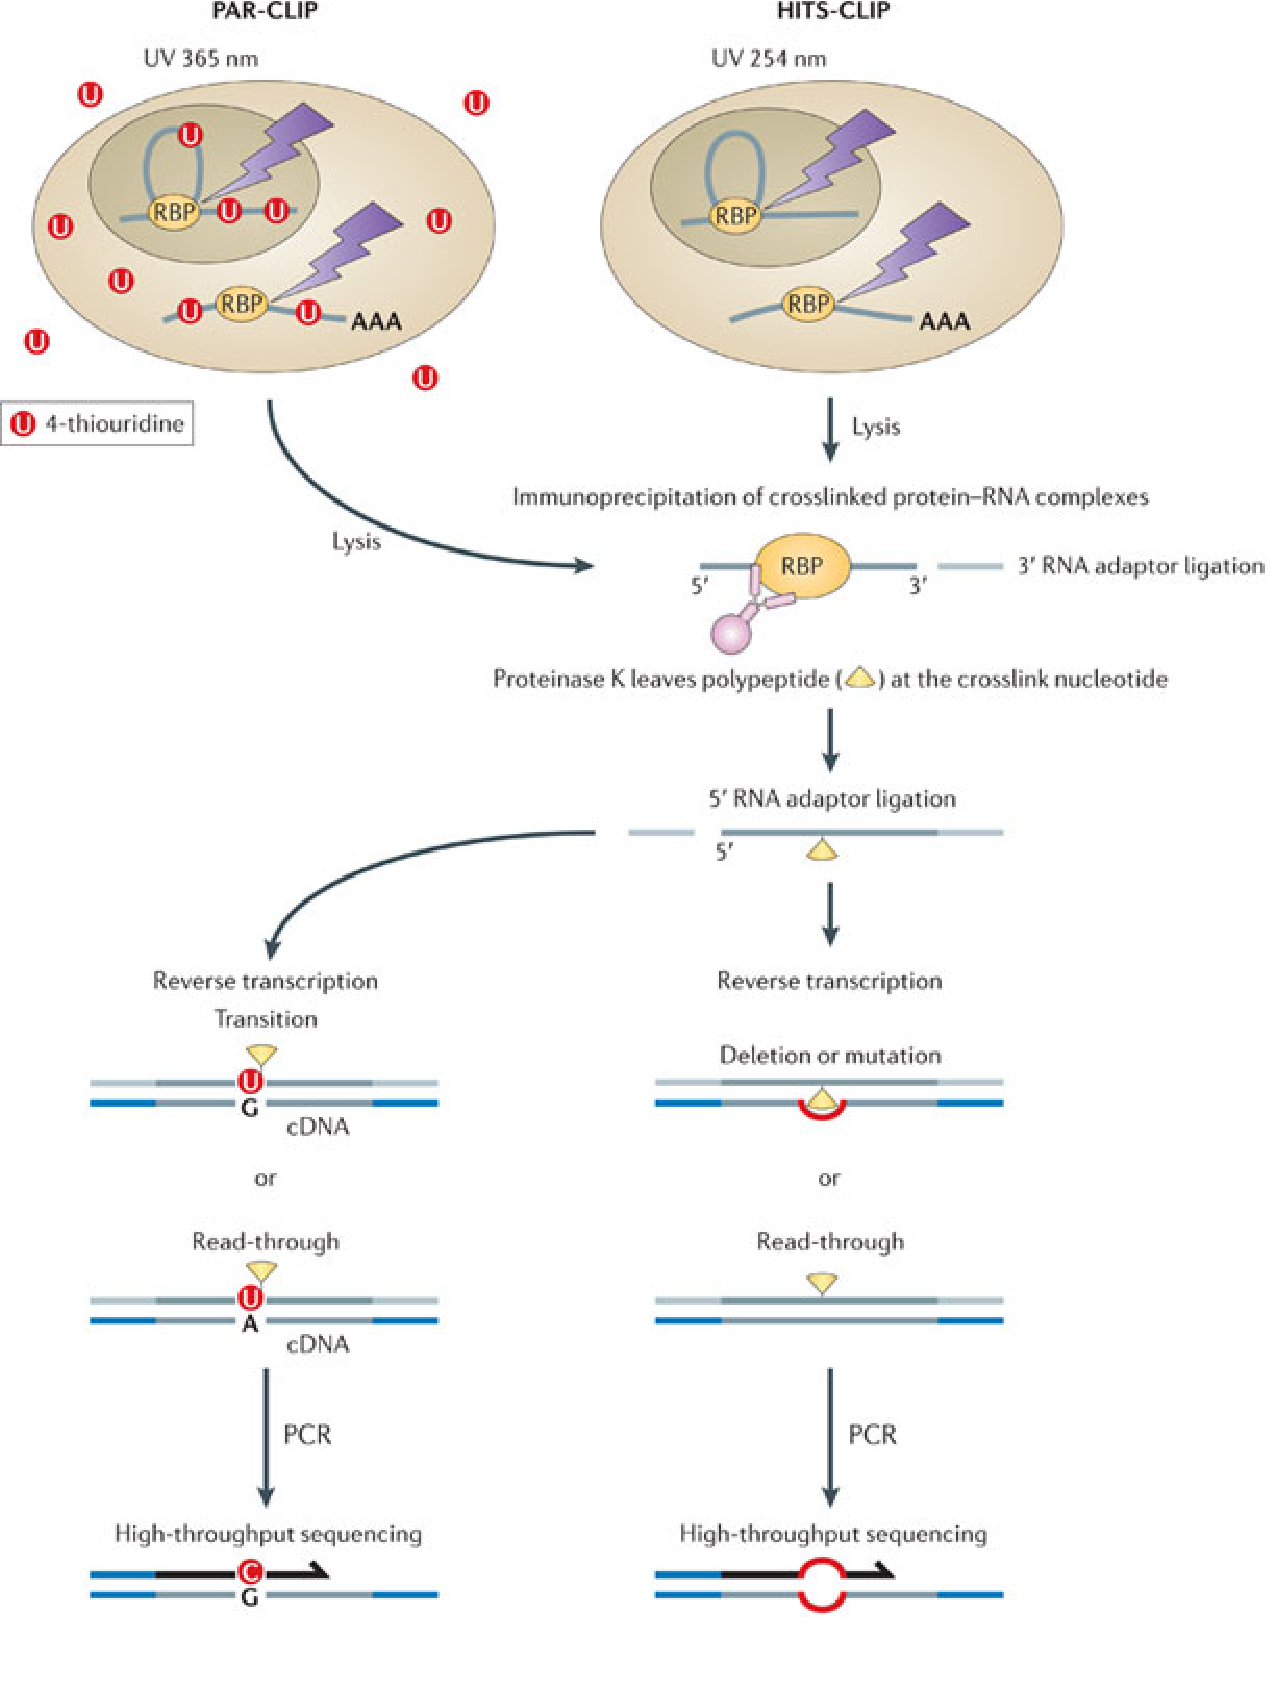
\includegraphics[width=0.5\textwidth,clip]{ch2_background/figures/parclip_hitsclip.pdf}

\caption[Various steps in PARCLIP and HITS-CLIP methods]{Various steps in PARCLIP and HITS-CLIP methods (Figure and description adopted from König et al. \cite{konig_2012})}
\label{PARCLIP_HITSCLIP}
\end{figure}
%\shorthandon{=}

\subsection{In silico methods} 

DNA motif finding tools such as MEME \cite{bailey_06} and HOMER \cite{heinz_2010} are commonly used to identify the binding motifs from a set of RNA sequences that are known to be bound by the RBP. Recently, several methods have been developed to specifically infer RNA motifs that include both sequence and structure features \cite{kazan_10, hiller_06, maticzka_14}. However, all of these methods require a set of bound RNA sequences so that they are based on the results of experimental methods.

De novo prediction of RBP-RNA interactions have been also studied. Pancaldi et. al. \cite{pancaldi_2012}, used more than 100 features such as 3’UTR characteristics, di-nucleotide content, RBP properties, RNA secondary structure statistics to predict the target mRNAs of RBPs in yeast. Muppirala et. al. \cite{muppirala_2011} developed a method called RPIseq that uses the 4-mer composition of the RNA sequence and the 3-mer composition of the RBP sequence to train a statistical model. They try both Support Vector Machine (SVM) and Random Forest (RF) methods to predict whether the RNA-RBP pair will interact or not. These methods have not been tested on a large dataset that contains human RBPs. 


\section{MicroRNAs}

MiRNAs are small (~22 nt long) non-coding RNAs that function in various biological pathways. They regulate gene expression by binding to target mRNAs containing complementary sequences. Recent studies show that over half of the human transcripts are subject to miRNA regulation through degradation or translation inhibition \cite{bartel_2009}. Studies have proved the effect of miRNAs on various cancer types, such as breast, lung, and prostate cancer. They are also implicated in some neurological disorders including schizophrenia and Alzheimer's diseases.

The first miRNA, lin-4, was discovered in \textit{C.elegans} \cite{lee_1993}. The identification of initial miRNAs led to extensive researches which resulted in the rapid discovery of many miRNAs. Currently, there are hundreds of miRNAs in the human genome.

MiRNAs bind to their target sites in 3'UTR of target mRNAs by either complete or partial complementary base pairing. The base pairing usually happens in the 5'-end of the miRNAs. This region is positioned at 2-7 nt of miRNAs and named as the 'seed region'. Complete complementary base pairing in this region is sufficient to downregulate the target mRNA. On the other hand, partial complementary in this region is compensated with additional base pairing in the 3'-end of the miRNAs. Similar to RBP-mRNA interactions, the interactions between miRNAs and mRNAs can be seen as a many-to-many relationship. A miRNA can bind to hundreds of mRNAs and an mRNA can contain target sites of several miRNAs. In the following section, we will briefly introduce the methods to identify miRNA targets.


\subsection{Methods for identification of miRNA binding sites}

Techniques such as qRT-PCR, luciferase reporter assays and western blot can be used to confirm an individual miRNA:mRNA interaction. qRT-PCR and western blot can be used to measure the downstream mRNA and protein expression changes upon the change of miRNA expression. However, these methods cannot distinguish between direct and indirect targets of miRNAs. Reporter assays, on the other hand, can prove a direct link by testing the effect of mutations in miRNA target sites. However, they are labor intensive. 

The methods described above can only be used to identify a small number of targets of the miRNA of interest. To identify the genome-wide targets of an miRNA, high throughput approaches have been also developed. One such approach is to measure the changes of gene expression upon miRNA transfection or inhibition. Microarray or RNA-seq techniques can be used to measure gene expression. One disadvantage of miRNA transfection method is that the miRNA of interest is expressed in higher than natural quantity. This can potentially saturate RISC complexes and affect the function of other endogenous miRNAs. MiRNA inhibition approach is also challenging because the antisense oligonucleotides that are used to inhibit the miRNA may not be specific enough to distinguish between the members of the same miRNA family. These methods still give a good overview of miRNA targets. 

Biochemical approaches to find miRNA targets involve the immunoprecipitation of the RISC component using an antibody against the Argonaute protein \cite{karginov_2007}. Precipitates are then analyzed either by microarray or sequencing to identify the targets. Similar to the identification of RBP sites, cross-linking by ultraviolet radiation technique can also be used here to identify miRNA sites. For instance, PARCLIP has been applied in HEK293 cells \cite{hafner_10}.

The approaches described so far analyze the effects of miRNAs on mRNAs. Measuring the change in protein expression is also important. Stable isotope labelling with amino acids in cell culture (SILAC) is one such method to measure protein abundance using mass spectrometry of samples labelled with different isotopes.


%Genetic methods identify miRNA binding sites through phenotypic suppression tests. The idea behind this approach is to find genes where mutations in miRNA sites rescue the loss of function phenotype of the miRNA. For example, a mutation in lin-41 rescued the bursting vulva phenotype of lethal 7 (let-7) mutant in \textit{C.elegans} \cite{reinhart_2000}. As such, this study shows that lin-4 is a target of let-7. Targets identified by this approach are physiologically relevant; however, the experimental protocol is laborious. As such, they can identify only a few targets of a miRNA. Also, it is not possible to distinguish between direct and indirect miRNA sites with these methods.

%Another approach to identify miRNA binding sites is to use biochemical methods. Initial methods of this kind aimed to isolate the sequence associated with miRNAs using Immunoprecipitation (IP) followed up by microarray or next generation sequencing (NGS) to identify miRNA target sites. Later, researchers took advantage of CLIP methods such as HITS-CLIP and PARCLIP to identify miRNA binding sites. MiRNAs are bound by Argonaute proteins (AGO1-4). Hafner et al. identified miRNA binding sites using PAR-CLIP approach by detecting AGO protein sites . We have discussed these identification methods in the RBPs section. 

MiRNA targets that have been identified by experimental methods are stored in databases. MirTarbase is one such database that contains more than fifty thousand experimentally validated miRNA-target interactions which are compiled by data-mining existing literature \cite{mirtarbase}. Interactions can be validated by several techniques such as reporter assay, western blot, northern blot, qRT-PCR, microarray, pSILAC and NGS based techniques. 

MiRNA targets have been initially determined by time-consuming low-throughput experiments. In the absence of high-throughput experiments, computational methods have been developed to predict miRNA targets. TargetScan is one of the most widely used method which considers complementarity to seed region and conservation information to predict miRNA target sites \cite{targetscan_05}. TargetScanS extends TargetScan by also taking into account other metrics such as local A-U content, target site position, target abundance, seed pairing stability, 3’ contribution. PicTar is another computational method that first assigns a probability to potential target sites based on base-pairing to seed region and conservation. These probabilities are then used in a hidden Markov model (HMM) to calculate the probability of generating the 3’UTR region by states that correspond to miRNA binding sites or background \cite{pictar_05}. GenMiR integrates matched mRNA-miRNA expression data into a Bayesian probabilistic model to predict miRNA targets \cite{genmir_2007} The likelihood of this model is calculated by a linear model that models the change in the expression level of potential targets to the expression of targeting miRNAs. GenMiR starts from an initial network of miRNA-mRNA targets that are predicted by TargetScan.

The regulatory effect of miRNAs depends on several factors. First, the location and secondary structure of binding sites may enhance the chance of miRNAs to bind to their targets. Studies show that AU-rich regions and unstructured areas such as 3'UTRs are more likely to be miRNA binding sites. Second, the number of miRNA binding sites plays a crucial role in the regulation of mRNAs. The more binding sites a transcript contains, the higher probability that it will be extensively regulated. Besides, miRNAs may involve in collaboration and competition interactions with RBPs. So far, most of the studies investigated the effect of one of these factors independently. However, recent studies show that miRNAs and RBPs are involved in complex gene regulation mechanisms. In the following sections, we first introduce RNA secondary structure which is important in recognition of binding sites of miRNAs and RBPs. Next, we briefly review previous work on the cooperative and competitive interactions between miRNAs and RBPs.

\clearpage
\section{RNA secondary structure}

A single-stranded RNA molecule can fold back onto itself forming a secondary structure. The most common base-pairs are the Watson-Crick base pairs A-T and G-C and the G-U wobble pair.

%\shorthandoff{=}
\begin{figure}[H]
   \centering
   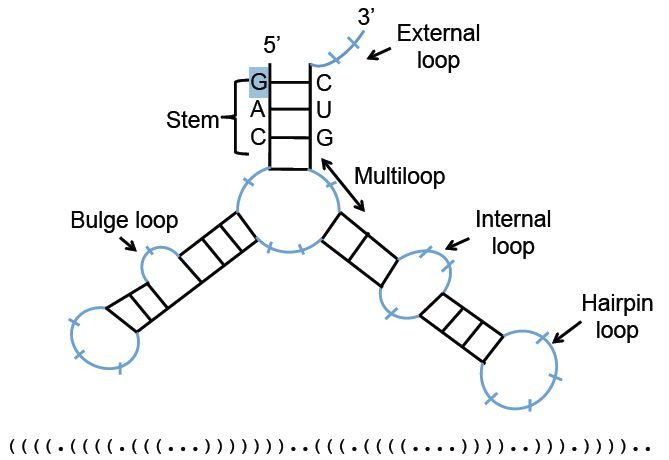
\includegraphics[width=0.8\textwidth,clip]{ch2_background/figures/secondary_structure}

\caption[Example of RNA Secondary Structure]{An RNA secondary structure example. One or more consecutive base pairs form a stem. Unpaired bases form various kinds of loops (shown in blue).}
\label{secondary_structure}
\end{figure}
%\shorthandon{=}

We can represent RNA secondary structure formally by assigning an index to each base in the RNA sequence. For example, we can start from the left end of the RNA sequence (5’end) and index each base by proceeding to the right end (3’end). If we assume that the indexing starts from 1 and the length of the sequence is N, a secondary structure S can be defined as a set of pairs i-j, 1 <= i < j <= N where each base is only paired with at most one other base. A stack of base pairs is called a stem.

Figure \ref{secondary_structure} shows an example secondary structure. Unpaired regions that are enclosed by one or more base pairs are called loops. They are several kinds of loops according to the number of closing base pairs. A hairpin loop is a circular end to a hairpin stem and it happens when there is a single closing base pair. A bulge or internal loop happens when there are two closing base pairs. Multi-loops have more than two closing base pairs. Finally, an external loop happens when the unpaired bases are at the end of the sequence. The same structure is shown with a dot-parenthesis notation on the bottom of the figure. In this notation, a matching pair of parentheses indicates a base pair and a dot denotes an unpaired base. 

There are several experimental techniques to determine the secondary structure of a RNA. However, these methods are difficult and time-consuming. Besides, experimental methods are unable to characterize the structures of many RNAs because of their conformational flexibility and large size. There are also methods in which scientists use chemical probing to increase the accuracy and the throughput of probing experiments \cite{kertesz_2010, FragSeq_2010, SHAPEseq_2011}. The basic idea behind this method is to use chemical reagent which leaves and imprint on the RNA molecule. These imprints can then be used to distinguish paired and unpaired nucleotides. These experiments, however, only report partial information of the structure.

There are three general categories for RNA secondary structure prediction algorithms: (i) comparative methods that infer the secondary structure common to aligned sequence across conserved species; (ii) thermodynamic methods that predict the structure with the minimum free energy (MFE); and (iii) probabilistic models that use parameters learned from known structures to predict unknown structures.

The comparative approach is most accurate when several aligned homologous RNA sequences are available \cite{gardner_04}. The disadvantage of this approach is that it is limited to datasets where the sequences are similar enough to get a reliable alignment. Therefore, these methods are not suitable to determine the secondary structure of all \textit{in vitro} and \textit{in vivo} data sets for any organism.

The second approach for discovering secondary structure is to use a set of thermodynamic parameters that predict the folding free energy of a given structure and a dynamic programming algorithm to find the structure with minimum free energy \cite{mathews_1999, mathews_06}. The idea behind this approach is that RNAs fold to the structure with the minimum free energy. One of the disadvantages of this approach is that an RNA molecule can fold into multiple structures during its lifetime. Therefore, the predicted MFE structure may not be the real, functional structure. One possible solution to address this issue is to consider the distribution of possible structures.

RNAfold is a method of this kind which computes probabilities for every possible base pair from the partition function. RNAplfold is a variant of RNAfold which uses local folding instead of global folding. This method considers base pairs within a certain span and calculates average base pair probabilities by averaging over all windows of a certain length that contain the pair. Studies show that this method performs more accurate than the classic global folding algorithms \cite{lange_12}. This algorithm uses little amount of memory and CPU time to run and therefore it is practical to scan large scale of the genome for short RNA structure.

SFOLD generates a statistical sample of RNA secondary structures from the Boltzmann ensemble of RNA secondary structures \cite{sfold}. Individual structures that are sampled by SFOLD can be used to calculate various probabilities such as probability of a region to form a stem with another region. 

Probabilistic models use parameters estimated from known RNA structures to predict secondary structure. There is also a method, called SimFold, which combines thermodynamic parameters and probabilistically estimated parameters \cite{andronescu_10}. These methods are becoming more powerful due to the increasing availability of known RNA structures.


\section{Competition and collaboration between RBPs and miRNAs}

Recent studies show that the RBPs and miRNAs, two major classes of post-transcriptional regulators, do not act independently. Instead, they are involved in competitive or cooperative interactions with each other. As such, the net outcome of target mRNA expression relies heavily on the interplay between these two classes of trans-acting factors. Here, we review some examples of these interactions.

\subsection{Collaboration between RBPs and miRNAs}

Jing et al. investigated the collaborative interaction between TTP and miR-16 which leads to the degradation of their target COX-2 mRNA \cite{jing_2005}. Both of these factors target the same AU-rich element (ARE) and as such, they are involved in direct interaction. In this study, they discovered that TTP interacts with miR-16 through association with AGO protein which assists miR-16 to bind to its target site. This process enables miR-16-mediated repression of COX-2 mRNA.

Interactions of HuR with miRNAs have been extensively studied as well. Kim et al. \cite{kim_2009} show that HuR and let-7 miRNA have to act together to repress translation of their target mRNA c-MYC. These two trans-acting factors repress c-MYC through an interdependent mechanism. In this study, they mutated the let-7 interaction sites and compared it with the wildtype case. They observed that segments with mutated let-7 sites did not respond to HuR silencing enhancement. On the other hand, they show that HuR is necessary for let-7 interaction with c-MYC mRNA. However, the underlying mechanism is still unclear. They suggest that HuR binding might change the local RNA structure, unmasking the let-7 recognition site.

Another interesting example is the cooperative interaction between the RBP PUM1 and the miRNAs miR-221/222 on the 3’UTR of the tumor suppressor gene p27 \cite{kedde_10}. Figure \ref{pum_miR-221} illustrates the binding sites of PUM1 and miR-221/222 on two sides of a same stem-loop. Binding of PUM1 protein alters the secondary structure and allows miR-221/222 to bind to the other side of the stem-loop. The cooperative interplay between these two factors leads to faster downregulation of p27.

%\shorthandoff{=}
\begin{figure}[H]
   \centering
   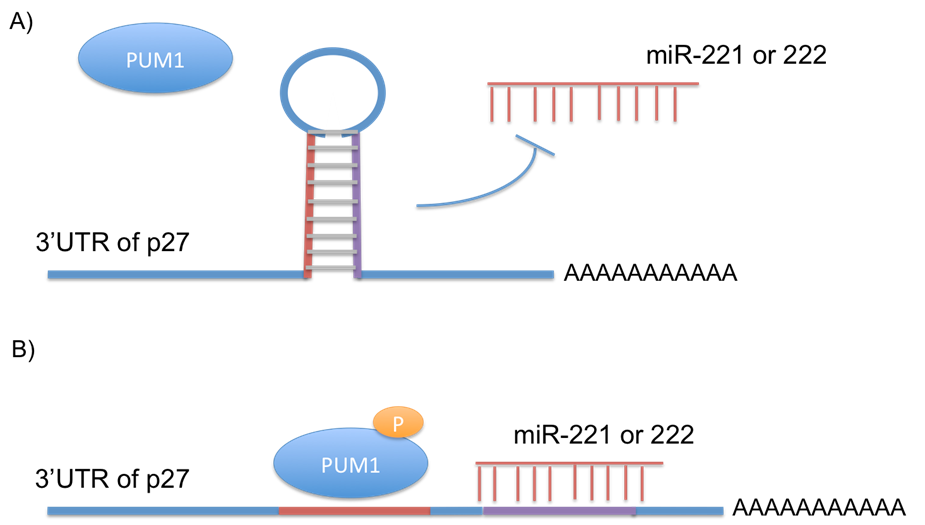
\includegraphics[width=0.8\textwidth,clip]{ch2_background/figures/pum_miR221.pdf}

\caption[Cooperative interaction between PUM1 and miR-221/222]{Cooperative interaction between PUM1 and miR-221/222.}
\label{pum_miR-221}
\end{figure}
%\shorthandon{=}

Figure \ref{pum_miR-221} shows the collaboration between PUM1 and miR-221/222. Without the PUM1, miR-221/222 is unable to bind to its target on p27 mRNA. Binding of PUM1 to its target in one side of the stem loop alters the secondary structure and makes it available for miR-221/222 to bind to the other side of the same loop. Their cooperation leads to faster degradation of their target mRNA.

\subsection{Competition between RBPs and miRNAs}

HuR has been shown to enhance the overall gene expression of both CAT-1 and COX-2 by protecting them from inhibitory action of miR-122 and miR-16, respectively \cite{bhattacharyya_2006, young_2012}. In the first case (CAT-1), HuR gets dephosphorylated and translocated from nucleus to the cytosol, where it binds to target ARE sequences on CAT-1 mRNAs and increases stability. This phenomenon leads to dissociation of miR-122 containing RISCs from CAT-1 mRNAs. Indeed, researchers also show that HuR is also able to displace the already bound RISCs. In the second case, HuR and miR-16 target the same ARE on COX-2 mRNA. In colorectal cancer cells, HuR gets overexpressed and localizes to the cytoplasm \cite{young_2012}. Under these conditions miR-16 is unable to promote mRNA decay. HuR is shown to directly associate with miR-16; however how HuR antagonizes miR-16 is still unclear. 

Another example of competition between RBPs and miRNAs is the translocation of the RBP HNRNPL under hypoxia conditions to compete with several miRNAs, including miR-297 or miR-299, on VEGFA 3’UTR through a CA-rich element. Binding of HNRNPL relieves VEGFA mRNA from miRNA-mediated repression.

The examples mentioned above provide a summary of known interactions between RBPs and miRNAs. Given the number of existing RBPs and miRNAs, these interactions constitute only a minority of the existing interactions between RBPs and miRNAs. These studies have focused on a single RBP or a single miRNA as laborious experiments are needed to confirm the interactions. Computational studies that scan for interactions between all RBPs and miRNAs can guide experimental studies. In the following section, we introduce two studies which aim to investigate combined effect of multiple factors in PTR.

\subsection{High-throughput techniques considering several factors}

Mukharjee et al. analyzed the combinatorial regulation by HuR and miRNAs \cite{mukharjee_11}. They investigated the condition in which binding sites of HuR and miRNAs overlap with each other. Their findings show that the existence of overlapping HuR sites relieves miRNA-mediated repression. However, the existence of overlapping miRNA sites has no effect in regulation mediated by HuR protein. This indicates that HuR is likely to compete with miRNAs for binding sites and stabilizes the targeted mRNAs.

In another study, researchers analyzed the effect of possible interactions between a few RBPs and miRNAs \cite{jiang_13}. They investigated the positional relationship of motif occurrences and observed that a particular RBP and an miRNA may interact with each other when there is a specific distance between their binding sites. For example, they showed that specific miRNAs tend to bind near PUM binding sites. These miRNAs have recognition seeds that are reverse complementary to the PUM recognition motifs. They show that PUM increases the accessibility of the sites for its interacting miRNAs which results in cooperation to promote mRNA decay. MiR-101, miR-300, miR-144, miR-221/222 are some examples of miRNAs that are predicted to interact with PUM. This is in accordance with the previous paper we described above, in which miR-221/22 pairs up with the PUM recognition sequence and cooperate with this protein to repress their target mRNA. 

Most of the previous studies have ignored the effect of RNA secondary structure whereas it is important in recognition of binding sites of RBPs and miRNAs. It is also beneficial to take advantage of existing knowledge on RBP binding, miRNA binding and mRNA stability by compiling CLIP datasets, experimental miRNA targets and genome-wide datasets of knockdown or transfection experiments. To the best of our knowledge, a comprehensive study of cooperative and competitive interactions between pairs of factors (i.e., all RBPs and miRNAs) is still lacking. In this thesis, we aim to investigate RBPs and miRNAs cooperative and competitive interaction comprehensively. First, we map the binding sites of RBPs and miRNAs on human 3’UTRs. Next, we utilize this comprehensive collection of sites to investigate interplay between each pair of factors and to predict half-life and mRNA abundance by considering effects of both RBPs and miRNAs.

